\chapter{Navigation \& Motor Control}

\section{Motor Controls}

\subsection{Overview}

The motor control subsystem governs the movement of the vehicle and is implemented within a single software file. It receives input from the pathfinding algorithm and translates this into control signals for the two on-board motors. The original motors are retained, and no modifications to the chassis are required.

\subsection{Hardware Architecture}

The motor control subsystem consists of two DC motors: a rear-mounted drive motor responsible for propulsion and a front-mounted motor used for steering via wheel pivoting. This configuration is retained from the original chassis design, avoiding physical modifications and ensuring compliance with project requirements on chassis dimensions. Maintaining the existing layout also reduces mechanical complexity and ensures compatibility with the pre-defined mounting structure.

Motor control is achieved using an L298N Dual H-Bridge Motor Driver Module, which provides an interface between the ESP32 microcontroller and the motors. The driver enables bidirectional control of each motor using an H-bridge configuration, allowing both forward and reverse operation.

The ESP32 supplies control signals to the driver through four digital input pins, which determine the direction of rotation for each motor. These input pins are arranged in pairs, with IN1 and IN2 controlling the steering motor, and IN3 and IN4 controlling the drive motor. By setting one pin in each pair high while the other is low, the polarity of the voltage applied to each motor is controlled.

The mapping between ESP32 GPIO pins and motor driver inputs is shown in Figure~\ref{fig:gpio_mapping}. In the implemented control scheme, each GPIO pin is associated with a specific vehicle movement command. Before a new command is issued, all motor control pins are driven low, ensuring that only one control signal is active at a time. This simplifies direction control and prevents conflicting input states from being applied to the motor driver.

\begin{figure}[h]
  \centering
  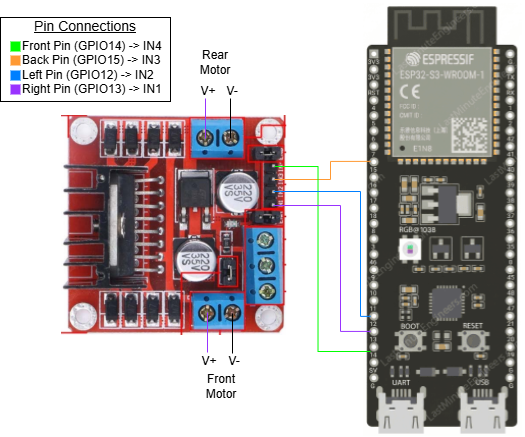
\includegraphics[width=0.7\textwidth]{images/ESP32MotorPinout.png}
  \caption{Mapping between ESP32 GPIO pins and motor driver inputs}
  \label{fig:gpio_mapping}
\end{figure}

Speed control is achieved using Pulse Width Modulation (PWM) signals generated by the ESP32 and applied to the enable pins of the driver. As the control signals are digital, the amplitude of the PWM signal remains constant, and motor speed is regulated by adjusting the duty cycle.

The L298N module is powered separately from the ESP32 logic supply, providing sufficient current to drive the motors. While the ESP32 operates at 3.3~V logic levels, the driver is compatible with these signals, enabling direct interfacing without additional level shifting circuitry.

\subsection{Control Logic}

The motor control system is implemented using four PWM channels, each corresponding to one input pin of the motor driver (IN1--IN4). At system initialisation, the \texttt{Motors\_Init()} function is called, configuring all PWM signals with a duty cycle of 0\%, ensuring that no motors are driven by default.

When the \texttt{Motors\_Apply()} function is invoked, control inputs from the pathfinding module are used to update the duty cycles of the relevant PWM channels. The order of operations is illustrated in Figure~\ref{fig:control_flow}.

\begin{figure}[h]
  \centering
  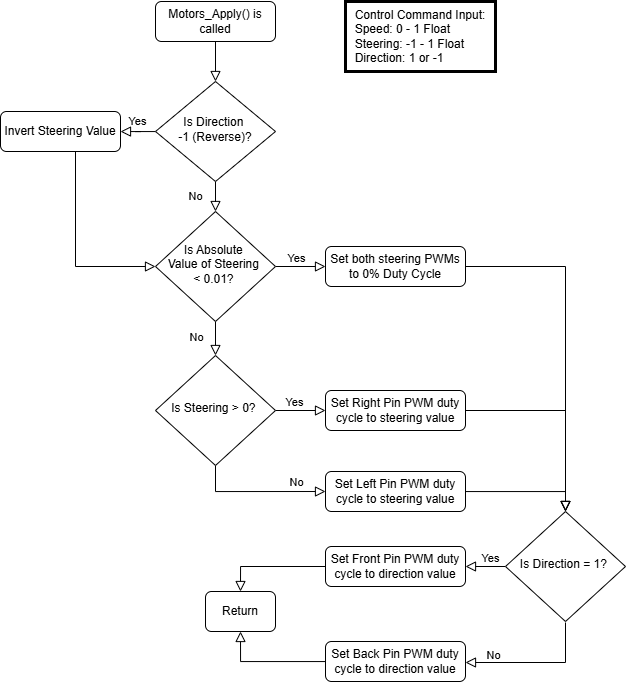
\includegraphics[width=0.7\textwidth]{images/MotorLogic.png}
  \caption{Motor control logic flow}
  \label{fig:control_flow}
\end{figure}

A non-zero duty cycle is applied only to the PWM channel corresponding to the desired direction of motion, while the complementary channel in the input pair remains at 0\%. This ensures that only one control signal is active for each motor at any time, preventing conflicting inputs from being applied to the motor driver.

Steering and propulsion are handled independently. The steering input determines which of the steering-related PWM channels is activated and to what duty cycle, while the direction input determines which propulsion-related channel is driven. This structure allows high-level motion commands to be translated directly into low-level motor control signals.

The control logic begins by evaluating the direction input. If the direction is negative (reverse), the sign of the steering value is inverted. This is required because the pathfinding algorithm defines steering relative to the forward-facing orientation of the vehicle; when reversing, the steering response must be inverted to achieve the intended motion.

Following this, the steering value is evaluated to configure the steering PWM outputs. To prevent unintended drift caused by very small floating-point values, a deadband is applied. If the magnitude of the steering input is below 0.01, both steering PWM channels are set to a duty cycle of 0\%. If the value is positive, the vehicle steers right; if negative, it steers left.

Finally, propulsion is configured by evaluating the direction input and applying the speed value to the corresponding PWM channel. This step is performed after steering configuration to ensure that the wheels are correctly oriented before motion begins. This ordering reduces the likelihood of incorrect movement if an interrupt occurs during execution of the \texttt{Motors\_Apply()} function.

\subsection{Software Implementation}

The motor control subsystem is structured as a modular interface consisting of three primary functions: \texttt{Motors\_Init()}, \texttt{Motors\_Apply()}, and \texttt{Motors\_Stop()}. This structure provides a clear abstraction layer between the motor control logic and the higher-level finite state machine.

The \texttt{Motors\_Init()} function is responsible for configuring the PWM channels used to drive the motor driver inputs. PWM generation and duty cycle control are implemented using the ESP32 LEDC library. All PWM channels are initialised with a duty cycle of 0\%, ensuring that the motors remain inactive on system startup.

The \texttt{Motors\_Apply()} function implements the control logic described in the previous section and serves as the main interface for motor control. It receives speed, steering, and direction inputs from the pathfinding module and translates these into PWM duty cycles applied to the motor driver inputs.

Input validation is performed within this function to ensure robust operation. Speed is constrained to [0, 1], steering is constrained to [-1, 1], and out-of-range values are clamped before applying PWM. The direction input is expected to be either -1 or 1; invalid values default to forward motion. This behaviour is intentionally chosen to prioritise forward displacement in the event of unexpected pathfinding outputs, maximising progress through the course while minimising reverse motion that does not contribute to overall advancement.

The function updates the PWM outputs by mapping validated input values directly to duty cycles, ensuring that only the channel corresponding to the intended direction of motion is active at any given time. This maintains consistency with the control scheme described previously and prevents conflicting motor commands.

The \texttt{Motors\_Stop()} function provides a simple mechanism to halt all motor activity by setting the duty cycle of all PWM channels to 0\%. This function is used both during testing and as a safety mechanism during operation.

\subsection{Testing}

The motor control subsystem was validated using a dedicated test driver, which repeatedly invoked the \texttt{Motors\_Apply()} function with predefined input values. These inputs were selected to cover both standard operating conditions and edge cases near decision thresholds within the control logic.

Each test case was executed on the physical hardware for a duration of 2 seconds, followed by a 0.5 second pause. During this pause, the \texttt{Motors\_Stop()} function was called, ensuring that both motion and stopping behaviour were verified. This approach allowed the response of the motors to be clearly observed for each input condition.

Test cases included nominal inputs, such as full forward motion and directional steering, as well as edge cases involving small steering magnitudes and direction changes. Due to the physical nature of the system, results were validated through observation of motor behaviour, confirming that the vehicle responded in accordance with the expected direction and speed.

The test suite was structured into four categories: normal operation, boundary conditions on speed, boundary conditions on steering, and extreme input values. Normal tests verified expected behaviour for typical motion commands, including forward, reverse, and combined steering inputs. Boundary tests evaluated system behaviour at and beyond defined input limits (e.g.\ $\pm1.0$), ensuring stable operation near decision thresholds. Extreme tests used significantly out-of-range values to confirm that the system remained stable and did not produce undefined behaviour.

A representative subset of test cases is shown in Table~\ref{tab:motor_tests}, with the full test suite provided in Appendix~A.

\begin{table}[h]
\centering
\resizebox{\textwidth}{!}{%
\begin{tabular}{|l|l|p{4cm}|p{4cm}|c|}
\hline
\textbf{Test Name} & \textbf{Input Value} & \textbf{Expected Result} & \textbf{Actual Result} & \textbf{Passed?} \\
\hline

Forward Only & [0.9f, 0.0f, 1] & Car drives straight forward, 75\% speed & Car drives straight forward, 75\% speed & Yes \\
\hline

Left Only & [0.0f, -0.9f, 1] & Front wheels turn left at a medium rate & Front wheels turn left at a medium rate & Yes \\
\hline

Reverse Left & [0.0f, 0.9f, -1] & Car reverses and turns left at medium rate & Car reverses and turns left at medium rate & Yes \\
\hline

Forward Speed Edge Over & [1.01f, 0.0f, 1] & Car drives straight forward, full speed & Car drives straight forward, full speed & Yes \\
\hline

Forward \& Left Under & [0.99f, -0.99f, 1] & Car drives forward, turning left, almost full speed & Car drives forward, turning left, almost full speed & Yes \\
\hline

Extreme Back \& Right & [20.0f, -20.0f, -1] & Car reverses right at full speed & Car reverses right at full speed & Yes \\
\hline

\end{tabular}
}%
\caption{Motor control test results}
\label{tab:motor_tests}
\end{table}

\section{Sensors and Sensor Management}
\subsection{Overview}

The sensor subsystem provides the environmental awareness needed by the navigation logic and the finite state machine. Three classes of sensor are used:
\begin{itemize}
    \item \textbf{Infrared (IR) reflectance sensors:} Four sensors mounted at each corner distinguish the marble floor from the black boundary tape.
    \item \textbf{VL53L3CX Time-of-Flight (ToF):} A forward-facing distance sensor measures the range to obstacles directly ahead.
    \item \textbf{MPU-6050 Inertial Measurement Unit (IMU):} Supplies a drift-compensated yaw rate that the APF planner uses to damp steering oscillations.
\end{itemize}
The bias-compensation pipeline that stabilises the gyroscope yaw rate is described in Section~\ref{sec:imu_bias}, and the normalised \texttt{SensorData} contract consumed by navigation is introduced in Chapter~\ref{ch:software_arch}.

Coordination of the three sensor types is handled by the ranging manager (\texttt{ranging\_manager.c}/\texttt{.h}), which encapsulates sensor initialisation, FreeRTOS task lifecycle, cached measurement storage, and per-device health monitoring. The ranging manager provides:
\begin{itemize}
    \item \textbf{Queue-based event delivery:} Each sensor task packages its readings into \texttt{sensor\_event\_t} packets and delivers them through the queue described in Section~\ref{sec:rtos_tasks}.
    \item \textbf{Direct-query interface:} Functions \texttt{ranging\_manager\_get\_latest\_tof()}, \texttt{ranging\_manager\_get\_latest\_ir()}, and \texttt{ranging\_manager\_get\_latest\_imu()} allow synchronous reads of the most recent cached values.
    \item \textbf{Runtime control:} Functions \texttt{ranging\_manager\_pause()}, \texttt{ranging\_manager\_resume()}, and the \texttt{ranging\_manager\_set\_*\_poll\_rate()} family allow polling to be suspended or retuned without tearing down the underlying tasks.
    \item \textbf{Centralised configuration:} Define all hardware-facing parameters, including pin assignments, polling intervals, calibration constants, detection thresholds, and per-device enable flags in \texttt{sensor\_config.h}.
\end{itemize}

\subsection{Hardware}
\subsubsection{IR sensor}
\label{sec:ir_hardware}

The IR reflectance sensors are TCRT5000-based DAOKAI modules\footnote{\href{https://www.amazon.co.uk/dp/B0B2PHWQH2}{DAOKAI TCRT5000 IR reflective module four-pack}} (Figure~\ref{fig:ir_breakout}), each pairing a 950~nm emitter with a phototransistor on a small breakout. White surfaces pull the analogue output close to ground, while matte black tape lets it rise towards the supply rail. Only the analogue output (A0) is used; it is wired into the ESP32-S3 ADC channels listed in Chapter~\ref{ch:hardware_arch}.

\begin{figure}[h]
\centering
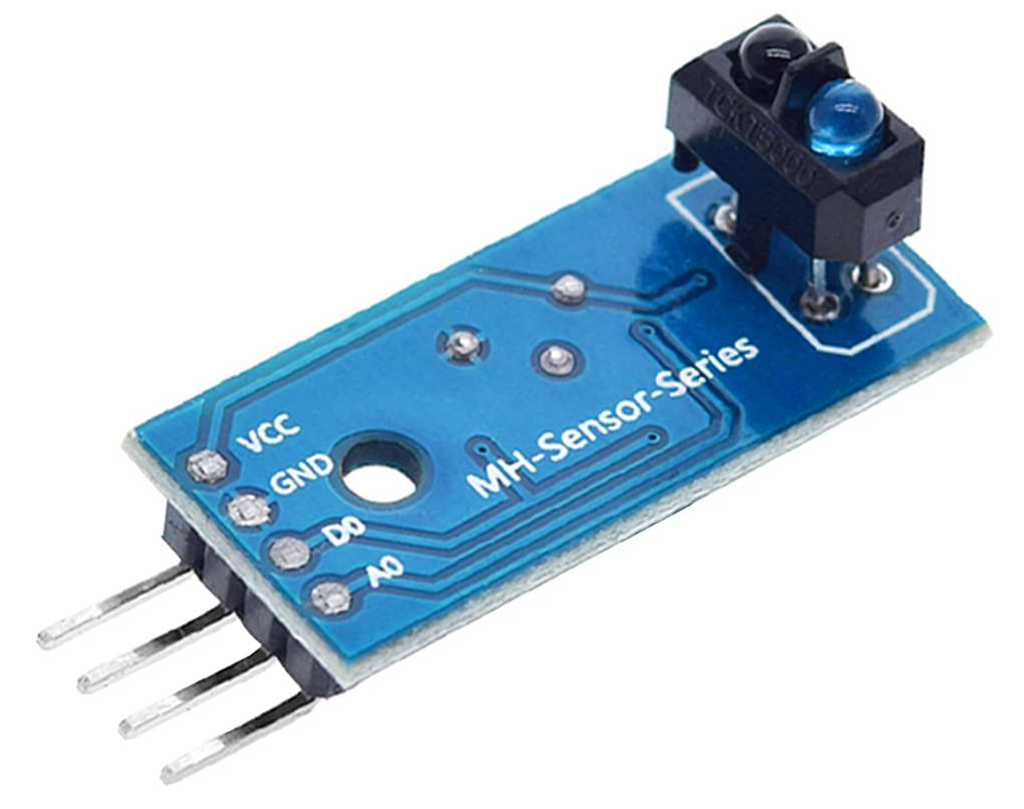
\includegraphics[width=0.5\textwidth]{images/ir_breakout.png}
\caption{TCRT5000 IR reflectance sensor module}
\label{fig:ir_breakout}
\end{figure}

A per-sensor linear mapping converts the calibrated voltage into a normalised tape ratio in the the range $[0.0, 1.0]$:
\[ r = \frac{V_{mv} - V_{blank}}{V_{tape} - V_{blank}} \]
where $V_{blank}$ and $V_{tape}$ are per-sensor calibration constants and the result is clamped before being passed to the navigation logic. 

The competition surface is polished marble with matte black boundary tape; both constants vary noticeably between corners due to mounting-height and unit-to-unit differences, so the defaults declared in \texttt{sensor\_config.h} are overridden at runtime with the values reported in the testing subsection.

The TCRT5000 datasheet specifies an effective sensing window of approximately 0.2--15~mm, and the analogue response depends strongly on the sensor-to-floor gap. The main practical limitations are:
\begin{itemize}
    \item \textbf{Mounting height:} small changes in the gap between the sensor and the floor cause large changes in the reading, so each sensor is calibrated separately.
    \item \textbf{Unit-to-unit variation:} the four breakouts do not give identical readings on the same surface, and the per-sensor calibration absorbs the difference.
    \item \textbf{Ambient light:} stray infrared light from outside can introduce noise and reduce the contrast between floor and tape.
    \item \textbf{Electrical noise:} the sensor has no on-board filtering, so noise from the motor driver can appear directly on the ADC input.
\end{itemize}
In practice, ambient lighting in the competition environment did not produce a measurable shift in the readings; bare-floor and on-tape voltages remained within calibration tolerance across the lighting conditions encountered during testing.

\subsubsection{ToF sensor}
\label{sec:tof_hardware}

Forward-facing ranging is provided by a Fermion VL53L3CX breakout from DFRobot\footnote{\href{https://thepihut.com/products/fermion-vl53l3cx-tof-distance-ranging-sensor-breakout}{Fermion VL53L3CX ToF distance ranging sensor breakout}} (Figure~\ref{fig:tof_breakout}) carrying the STMicroelectronics VL53L3CX module. The sensor combines a 940~nm Class~1 VCSEL emitter with a SPAD receive array and reports up to four targets per ranging frame, each with a status code indicating measurement validity.

\begin{figure}[h]
\centering
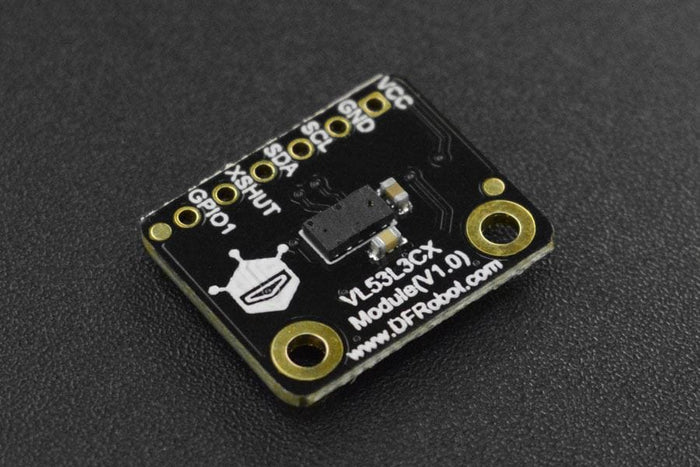
\includegraphics[width=0.5\textwidth]{images/tof_breakout.jpg}
\caption{Fermion VL53L3CX ToF ranging sensor breakout}
\label{fig:tof_breakout}
\end{figure}

The driver configures \texttt{VL53LX\_DISTANCEMODE\_MEDIUM} for improved ambient-light immunity at the cost of upper range. The main ranging loop takes the first valid target and converts it into centimetres before passing it to the navigation logic.

The VL53L3CX datasheet\footnote{\href{https://www.st.com/en/imaging-and-photonics-solutions/vl53l3cx.html}{STMicroelectronics VL53L3CX product page and datasheet}} notes the following limitations relevant to the application:
\begin{itemize}
    \item \textbf{Maximum range:} up to 310cm against an 88\% reflectivity target, dropping to 170cm against a 17\% target under low ambient light (i.e. indoors).
    \item \textbf{Field of view:} a typical $25^\circ$ FoV, sufficient for forward obstacle detection.
    \item \textbf{Minimum range:} reliable detection begins at approximately 25~mm; closer targets return either minimum detection range or invalid status codes, which the firmware treats as ``no target'' rather than zero distance.
\end{itemize}

\subsubsection{IMU sensor}
\label{sec:imu_hardware}

The inertial measurement unit is a DollaTek MPU-6050 breakout\footnote{\href{https://www.amazon.co.uk/dp/B07DJ4KMBF}{DollaTek MPU-6050 6-axis IMU breakout}} (Figure~\ref{fig:imu_breakout}) carrying the InvenSense MPU-6050. The application uses the gyroscope yaw axis for the APF damping term and the accelerometer purely as a stationarity detector for the bias-calibration logic in Section~\ref{sec:imu_bias}.

\begin{figure}[h]
\centering
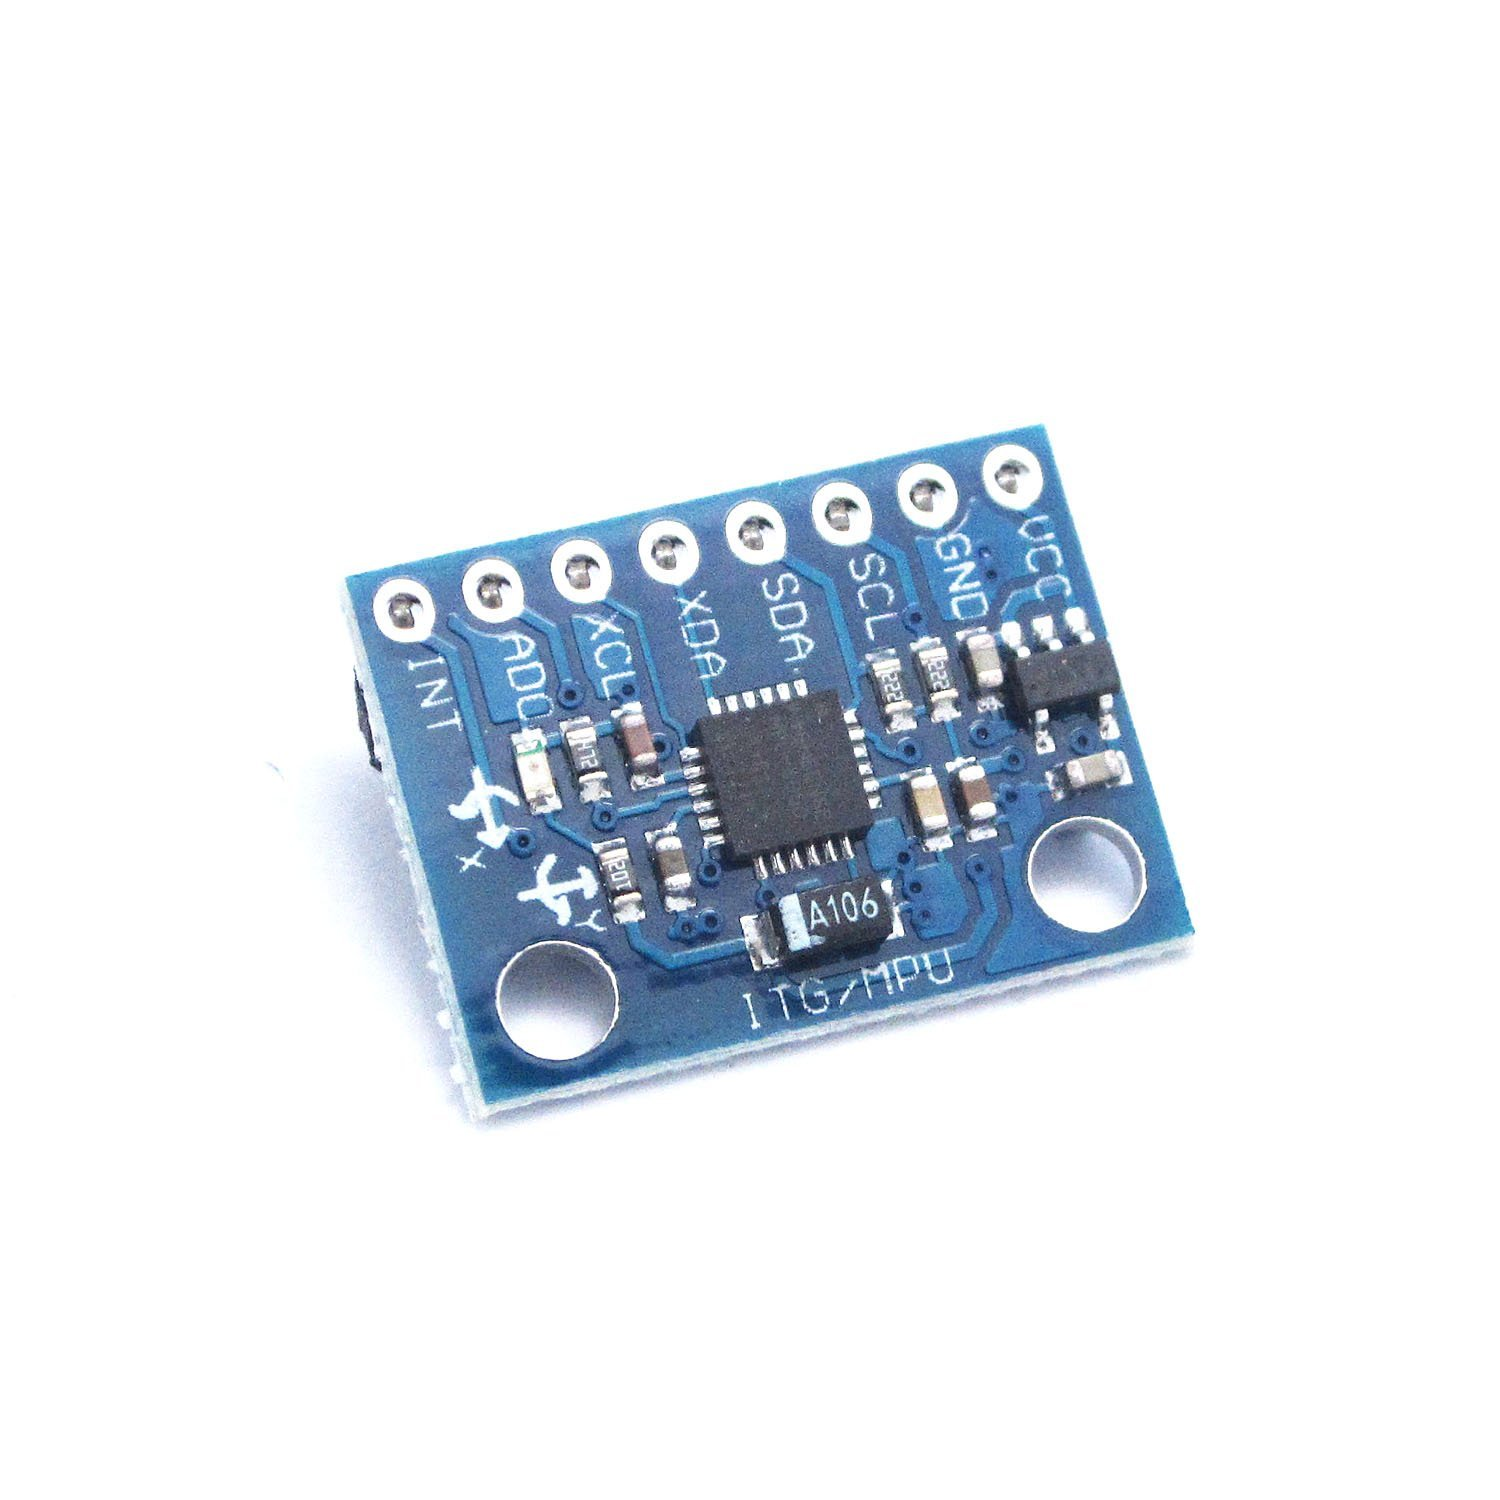
\includegraphics[width=0.5\textwidth]{images/imu_breakout.jpg}
\caption{MPU-6050 six-axis IMU breakout}
\label{fig:imu_breakout}
\end{figure}

The MPU-6050 datasheet notes the following limitations relevant to the application:
\begin{itemize}
    \item \textbf{Gyroscope zero-rate drift:} non-zero output varies with temperature and power cycle; compensated by the EMA bias estimator in Section~\ref{sec:imu_bias}.
    \item \textbf{Vibration sensitivity:} chassis vibration can briefly violate the $1g \pm 0.2g$ stationarity criterion and pause bias updates.
\end{itemize}

\subsection{Software}

The ranging manager polls each sensor on its own task and caches the most recent sample for synchronous readers.

\subsubsection{Architecture}

The ranging manager spawns one FreeRTOS task per enabled sensor type and uses \texttt{vTaskDelayUntil()} to hold each at its configured cadence (10~ms IR, 20~ms IMU, 30~ms ToF). Each iteration calls the driver, locks the shared mutex, writes the new sample into the cached \texttt{tof\_sample\_t}, \texttt{ir\_sample\_t}, or \texttt{imu\_sample\_t}, releases the mutex, and posts a \texttt{sensor\_event\_t} to the output queue. The cached samples are read by \texttt{ranging\_manager\_get\_latest\_*()}; the queue is drained by the main control loop.

Each task also updates a per-device health flag (\texttt{SENSOR\_STATE\_OK}, \texttt{\_ERROR}, or \texttt{\_OFFLINE}) that callers can read through \texttt{ranging\_manager\_get\_*\_health()}; the IR sensors are tracked per channel so the FSM can ignore one channel while still trusting the other three.

\subsubsection{Queue and Runtime Control}

The output queue is owned by the application and passed into \texttt{ranging\_manager\_start()}, which keeps queue lifetime decoupled from the manager. Producer-side sends are non-blocking: if the queue is full the oldest event is discarded and the new event is sent in its place, so a slow consumer cannot block a polling task and skew the IMU sampling interval. The consumer-side rate limiting that drains this queue is described in Section~\ref{sec:rtos_tasks}.

Runtime control is provided by \texttt{ranging\_manager\_pause()} and \texttt{ranging\_manager\_resume()}, which toggle a flag that each task observes at the top of its loop, and by the \texttt{ranging\_manager\_set\_*\_poll\_rate()} family, which adjusts the cadence taken by \texttt{vTaskDelayUntil()} on the following iteration without restarting the task. For the IR sensors, an additional \texttt{ranging\_manager\_ir\_tune()} hook allows the per-channel calibration constants to be updated at runtime, which was used during calibration to converge on the values reported in Section~\ref{sec:ir_calibration} without recompiling the firmware.

\subsubsection{Firmware}

The IR and ToF sensors each have a dedicated driver under \texttt{components/}; the ranging manager calls these drivers and does not access the hardware directly.

The IR driver (\texttt{components/ir\_driver/ir.c}) was written entirely in-house. It wraps the ESP-IDF \texttt{adc\_oneshot} and \texttt{adc\_cali} APIs behind a small per-sensor interface (\texttt{ir\_sensor\_init()}, \texttt{ir\_sensor\_read\_raw()}, \texttt{ir\_sensor\_read\_voltage()}, \texttt{ir\_sensor\_tape\_detected()}, \texttt{ir\_sensor\_deinit()}, and \texttt{ir\_tape\_ratio()}). Two aspects of the driver are worth noting:
\begin{itemize}
    \item \textbf{Reference-counted ADC unit handles:} static \texttt{adc\_oneshot\_unit\_handle\_t} instances for ADC1 and ADC2 are shared between channels and only torn down when the last sensor releases them, avoiding redundant re-initialisation as the four IR sensors are brought up sequentially.
    \item \textbf{Calibration with graceful fallback:} curve-fitting calibration via \texttt{adc\_cali\_create\_scheme\_curve\_fitting()} is attempted per channel, falling back to raw-count operation if eFuse data is absent and surfacing \texttt{ESP\_ERR\_INVALID\_STATE} so the caller can detect the missing calibration explicitly.
\end{itemize}

The ToF driver (\texttt{components/vl53l3cx\_driver/tof\_vl53l3cx.c}) is an in-house wrapper above the STMicroelectronics VL53L3CX BareDriver (STSW-IMG015\footnote{\href{https://www.st.com/en/embedded-software/stsw-img015.html}{STSW-IMG015 — VL53L3CX BareDriver}}). The vendor library handles register access, ranging-mode configuration, and on-chip calibration; the wrapper adds the bus and reset handling that the BareDriver leaves to the caller:
\begin{itemize}
    \item \texttt{tof\_vl53l3cx\_init()} runs the XSHUT reset, registers the device on the ESP-IDF \texttt{i2c\_master} bus, and drives the BareDriver bring-up sequence (\texttt{VL53LX\_WaitDeviceBooted}, \texttt{\_DataInit}, \texttt{\_SetDistanceMode}, \texttt{\_StartMeasurement}); any failure rolls back the I$^2$C registration.
    \item \texttt{tof\_vl53l3cx\_get\_data()} polls without blocking via \texttt{VL53LX\_GetMeasurementDataReady}/\texttt{\_GetMultiRangingData}/\texttt{\_ClearInterruptAndStartMeasurement}, returning \texttt{ESP\_ERR\_INVALID\_STATE} when no new frame is available so the ToF task can skip a cycle without holding the bus.
    \item \texttt{tof\_vl53l3cx\_deinit()} stops the measurement engine, asserts XSHUT, and removes the device from the bus.
    \item \texttt{vl53l3cx\_hardware\_reset()} applies the XSHUT timing required by the device datasheet.
\end{itemize}

The MPU-6050 is supported by an in-house driver under \texttt{src/imu\_util.c} that registers the device on the shared \texttt{i2c\_master} bus, performs power-management and range configuration, and exposes \texttt{imu\_setup()}, \texttt{imu\_teardown()}, \texttt{imu\_get\_who\_am\_i()}, and a polling routine returning an \texttt{imu\_sample\_t} (scaled accelerometer in $g$, gyroscope in deg/s, and die temperature). The driver is not packaged under \texttt{components/}; the heading estimator that consumes its output (\texttt{src/imu\_heading.c}) is described in Chapter~\ref{ch:software_arch}.

\subsection{Testing}

\subsubsection{IR Calibration}
\label{sec:ir_calibration}

The IR sensors were calibrated in place on the assembled vehicle on a polished marble floor with matte black boundary tape. The procedure for each sensor in turn was:
\begin{enumerate}
    \item Set $V_{blank}$ to a common approximate baseline (50~mV) representing the bare marble floor, rather than measuring it individually per sensor.
    \item Position the vehicle so that the sensor sat over the tape and log the steady-state ADC voltage as $V_{tape}$.
    \item Apply the new values at runtime through \texttt{ranging\_manager\_ir\_tune()} and only freeze them into \texttt{app\_main.c} once they were stable across multiple traversals of the tape.
\end{enumerate}

\begin{table}[h]
\centering
\begin{tabular}{|l|l|c|c|}
\hline
\textbf{Sensor} & \textbf{Position} & \textbf{$V_{blank}$ (mV)} & \textbf{$V_{tape}$ (mV)} \\
\hline
IR1 & Front Right & 50 & 290 \\
\hline
IR2 & Front Left & 50 & 1500 \\
\hline
IR3 & Rear Right & 50 & 2800 \\
\hline
IR4 & Rear Left & 50 & 2800 \\
\hline
\end{tabular}
\caption{Per-sensor IR calibration constants used at runtime}
\label{tab:ir_calibration}
\end{table}

The resulting per-sensor constants are summarised in Table~\ref{tab:ir_calibration}. The navigation logic acts on the normalised ratio $r$ defined in Section~\ref{sec:ir_hardware} rather than on a hard voltage threshold, so only $V_{blank}$ and $V_{tape}$ have functional effect; the per-channel \texttt{detect\_threshold\_mv} field exists in \texttt{ir\_sensor\_config\_t} but is currently used only by the debug log printer.

The front-right channel reports a tape voltage roughly an order of magnitude lower than the rear sensors; this was traced to a likely unit-to-unit variation between the four breakout boards rather than to mounting geometry, and the per-sensor mapping absorbs the difference without needing a hardware swap.

\subsubsection{Tests}

The sensor drivers were tested using two Unity test suites under \texttt{test/} running on the ESP32, together with a hardware-in-the-loop check on the assembled vehicle:
\begin{itemize}
    \item \textbf{\texttt{test\_ir\_util.c}:} covers invalid-argument handling, the setup and teardown lifecycle, the voltage and ratio conversion bounds, and the sharing of a single \texttt{adc\_oneshot} unit between multiple channels.
    \item \textbf{\texttt{test\_ranging\_manager.c}:} covers invalid-argument rejection on \texttt{ranging\_manager\_start()}, the start-to-stop lifecycle, queue delivery of \texttt{sensor\_event\_t} packets, and pause/resume behaviour.
    \item \textbf{In-loop testing:} the ToF and IMU drivers are tested by logging sensor readings to the serial output and checking that the values are plausible: the reported distance falls as the vehicle approaches a wall, the IR ratios saturate at the tape boundary, and the gyroscope yaw rate inverts when the vehicle is rotated by hand.
\end{itemize}

\subsubsection{Mock Sensors}

The ToF and IMU sensors each have a mock implementation (\texttt{src/tof\_mock.c} and \texttt{src/imu\_mock.c}) that satisfies the same function signatures as the real driver and returns synthetic but bounded samples. The mocks are selected at compile time through the \texttt{MOCK\_TOF\_SENSOR} and \texttt{MOCK\_IMU\_SENSOR} macros in \texttt{sensor\_config.h} and are used during firmware bring-up, before the I$^2$C bus has been brought online or when the corresponding physical sensor is unavailable, so that the FSM, the APF planner, and the ranging manager itself can be exercised without the full hardware stack.

\section{Path Planning}

\subsection{Overview}

The path planning subsystem is responsible for converting sensor data into motion commands for the vehicle. Unlike a map-based planner, this implementation uses an artificial potential field (APF) approach, in which the vehicle is guided by a combination of attractive and repulsive influences derived from the sensors. The resulting heading and speed are then passed into the motor control subsystem.

This method was chosen because it is compact, computationally efficient, and allows for a small non complete map to be used. The path planning logic operates directly on the inputs from the infrared and distance sensors along with the IMU data. By using continuous sensor feedback, the vehicle is able to react dynamically to changes in the environment while maintaining smooth motion.

\subsection{Sensor Interpretation and Field Construction}

The path planning algorithm uses four infrared (IR) sensors positioned around the vehicle, together with a front-facing time-of-flight (ToF) distance sensor and an inertial measurement unit (IMU). The IR readings are first clamped to prevent invalid values from influencing the navigation logic. These readings are then grouped into left, right, front, and rear loads, allowing the vehicle to estimate its location relative to nearby walls.

A measured wall heading is computed using the relationship:

\[\theta_{wall} = \arctan2(L - R, F - B)\]

where $L$ and $R$ represent the combined left and right sensor loads, and $F$ and $B$ represent the combined front and rear loads. This heading is wrapped to the range of $[-180^\circ, 180^\circ]$ to ensure the path planning outputs are possible for the vehicle to achieve.

The IMU is used to steady the APF output rather than define the navigation field itself. The drift-compensated yaw rate from Chapter~3 is fed into the planner to soften sharp steering changes and reduce the oscillation that can occur when the APF repeatedly rebounds from walls and black tape. When \texttt{imu\_heading\_valid} is set, the IMU heading can also nudge the stored wall reference, but IR and ToF data still provide the main navigation input.

During initialisation, the subsystem stores an \emph{original wall heading} as a stable reference direction. Once the ToF sensor reports a valid distance measurement, that heading is updated each cycle using the current IR balance and distance reading so the reference can adapt gradually to the course.
\subsection{Control Logic}

The navigation decision is based on the combination of attractive and repulsive fields. The attractive component encourages the vehicle to move in the direction of the stored wall heading, which acts as the intended course direction. Its magnitude is scaled according to the measured front distance, meaning that the vehicle is encouraged to move more strongly when there is sufficient space ahead.

Repulsive forces are generated from the IR sensor imbalance. These forces oppose proximity to nearby tape or obstacles and are calculated using the difference between the left and right sensor loads, as well as the front and rear loads. The repulsive field is then combined with the attractive field to produce a resultant vector representing the desired direction of travel.

The final heading is calculated from this resultant vector using:

\[\theta_{desired} = \arctan2(F_y, F_x)\]

where $F_x$ and $F_y$ are the horizontal and vertical components of the combined field. This approach allows the vehicle to balance course-following behaviour with obstacle avoidance in a single control step.

Speed is estimated from the magnitude of the resultant field and then adjusted according to environmental risk. Motion is reduced when the vehicle is close to a wall or obstacle, it is also reduced when the IR sensors indicate a strong tape danger signal. In addition, if the repulsive component becomes large, the maximum speed is capped to reduce oscillation and improve stability. This produces smoother behaviour in confined or ambiguous sections of the course.

To prevent abrupt changes in motion, the heading command is filtered using temporal smoothing by interpolating the new output with the previous heading. This reduces jitter and helps the vehicle maintain stable motion across successive control cycles.

\subsection{Software Implementation}

The path planning subsystem is implemented through two primary functions: \texttt{apf\_navigation\_init()} and \texttt{apf\_navigation\_compute()}. A third function, \texttt{apf\_navigation\_to\_control()}, converts the resulting navigation command into the format required by the motor control subsystem.

The \texttt{apf\_navigation\_init()} function resets the internal state variables used by the planner. These include the stored wall heading, a validity flag indicating whether the reference heading has been established, and the previous heading and speed values used for smoothing. Initialising these values ensures that the first navigation cycle begins from a known state.

The \texttt{apf\_navigation\_compute()} function contains the main APF logic. It receives sensor data, validates and clamps the inputs, computes the attractive and repulsive components, and produces a desired heading and speed. Internal memory is updated at the end of each call so that the next iteration can make use of the previous output. This stateful design is important because it provides continuity between control cycles and improves navigation stability.

The \texttt{apf\_navigation\_to\_control()} function maps the APF output into low-level drive commands. The heading is normalised to a steering range by dividing it by $40^\circ$ and clamping the result to $[-1,1]$. The speed value is also constrained to $[0,1]$. The direction output is fixed to forward motion, meaning that the planner is designed primarily for continuous forward navigation rather than reversing manoeuvres.

This separation between navigation and motor control provides a clear abstraction layer. The path planner determines \emph{where} the vehicle should move, while the motor control subsystem determines \emph{how} that motion is physically applied to the motors.

\subsection{Behavioural Characteristics}

The implemented APF strategy provides several useful behaviours. The vehicle tends to follow a stable course when the surroundings are consistent, because the original wall heading acts as a persistent directional reference. When the environment changes, the repulsive field helps prevent collisions or tape violations by steering the vehicle away from local hazards. The smoothing stage then prevents the output from changing too abruptly, which is particularly beneficial when sensor readings fluctuate between adjacent control cycles.

The use of a distance-based speed reduction also improves safety. When the vehicle approaches a wall or obstacle, the planner automatically slows the vehicle down, giving the steering system more time to respond. Similarly, strong IR activity near the tape causes the vehicle to reduce speed, lowering the likelihood of overshooting the course boundary.

Overall, the path planning subsystem provides a lightweight and reactive navigation method that is well matched to the available sensors and embedded processing platform. Its continuous control structure allows the vehicle to maintain progress while dynamically adapting to local obstacles and course constraints.

